\def\MyCourse{データサイエンスコース}
\def\MySubject{R入門}
\def\MySemester{春学期}

\newcommand{\R}{\textbf{R}}
\newcommand{\RStudio}{\textbf{RStudio}}
\newcommand{\Excel}{\textbf{Excel}}
\newcommand{\cs}[1]{\textcolor{blue}{\texttt{#1}}} % Console prompt >

\renewcommand{\include}[1]{}
\maketitle
\begin{frame}

\frametitle{目次}
\scriptsize
\begin{columns}[t]
    \begin{column}{.5\textwidth}
        \tableofcontents[sections={1-4}]
    \end{column}
    \begin{column}{.5\textwidth}
        \tableofcontents[sections={5-}]
    \end{column}
\end{columns}

\end{frame}

C:/Users/hss/AQUOS/Default_Folder/TIU/lectures/applied_stats/000-main.tex
\section{はじめに}
\def\MyCourse{データサイエンスコース}
\def\MySubject{R入門}
\def\MySemester{春学期}

\newcommand{\R}{\textbf{R}}
\newcommand{\RStudio}{\textbf{RStudio}}
\newcommand{\Excel}{\textbf{Excel}}
\newcommand{\cs}[1]{\textcolor{blue}{\texttt{#1}}} % Console prompt >


\mysffr

統計解析は,10年ほど前までは,CやFortranなど,取扱いに専門的知識を要する
プログラミング言語を用いて行われていました.
これを,高度なプログラミング知識がなくても誰でも利用できる形にしたものが,統計解析環境\R です.
今や,データサイエンスの世界では標準のソフトウェアツールとなっています.\\

\vspace{5mm}
\R を習得すれば,統計解析から業務効率化ツールの作成までオールマイティーに,
そのスキルを活用できます.
電力事業に携わる方は,様々な市販のソフトウェアに手を出さなくても,これ一本で十分です.
当社の重要なシステムも\R で動いています.

\vspace{5mm}
Learn by practice\\
\vspace{5mm}
手を動かして自分でやってみることが\R 習得の近道です.そのため,各スライドには,
必ず演習を載せてあります.\\


\end{frame}

\end{document}



\section{統計解析環境}
%
% Section title page as a seperator
%

\def\MyCourse{データサイエンスコース}
\def\MySubject{R入門}
\def\MySemester{春学期}

\newcommand{\R}{\textbf{R}}
\newcommand{\RStudio}{\textbf{RStudio}}
\newcommand{\Excel}{\textbf{Excel}}
\newcommand{\cs}[1]{\textcolor{blue}{\texttt{#1}}} % Console prompt >


\begin{frame}[fragile]
  \centering
  \Huge
  \insertsection 

\end{frame}

\end{document}


\def\MyCourse{データサイエンスコース}
\def\MySubject{R入門}
\def\MySemester{春学期}

\newcommand{\R}{\textbf{R}}
\newcommand{\RStudio}{\textbf{RStudio}}
\newcommand{\Excel}{\textbf{Excel}}
\newcommand{\cs}[1]{\textcolor{blue}{\texttt{#1}}} % Console prompt >


\subsection{\R}

\myffr

  \R とは,AT&Tベル研究所が開発した統計解析用の
  プログラミング言語(S言語)
  を参考にして作られたオープンソースの言語(R言語)を使用できる
  統計解析環境.
  \vspace{5mm}

 \begin{minipage}{0.45\hsize}
  \begin{figure}
    \centering
    
\includegraphics[width=0.3\linewidth]{logo-r}
    \label{fig:logo-r}
    \caption*{The R environment}
  \end{figure}
  \end{minipage}
  \hspace{3mm}
  \begin{minipage}{0.45\hsize}
  \begin{figure}
    \centering
    
\includegraphics[width=0.3\linewidth]{r-open}
    \label{fig:r-open}
    \caption*{Microsoft R Open}
  \end{figure}
  \end{minipage}

  \vspace{5mm}
  \R により,現代統計学をほぼ網羅する広範な統計解析や
  出版物品質のグラフ描画が容易に可能となる.

  \vspace{5mm}
  Microsoft社により開発・保守されている高速版の\R も存在する.

\end{frame}

\subsection{\R パッケージ}

\myffr

  \R だけでも基本的な統計解析は可能だが,
  ユーザーの利用目的に応じて開発された\R パッケージと呼ばれる
  統計解析ライブラリをインストールすることで機能を拡張できる.
  \vspace{5mm}
  
  \R パッケージは,C/C++,Fortran,R言語で記述されており,
  当初は,欧米大学の統計学科の教員らが中心となり
  開発・保守を行っていたが,
  近年は民間を含む様々な分野で広く開発が進められている.
  すでに,1,000を超える\R パッケージがインターネット上で公開されている.

\end{frame}

\subsection{CRAN}

\myffr

  CRAN(包括的R保存庫網)とは,\R の本体やパッケージ,
  マニュアル類が無償公開されているウェブサイト.
  ユーザーは,最寄りのミラーサイトからソフトウェアをダウンロードする.
  %\R 関連のソフトウェアをダウンロードする際には,
  %次の国内のサイトを利用する.

  %$\rightarrow$ 統計数理研究所(\url{https://cran.ism.ac.jp})

  \begin{figure}[h]
    \centering
    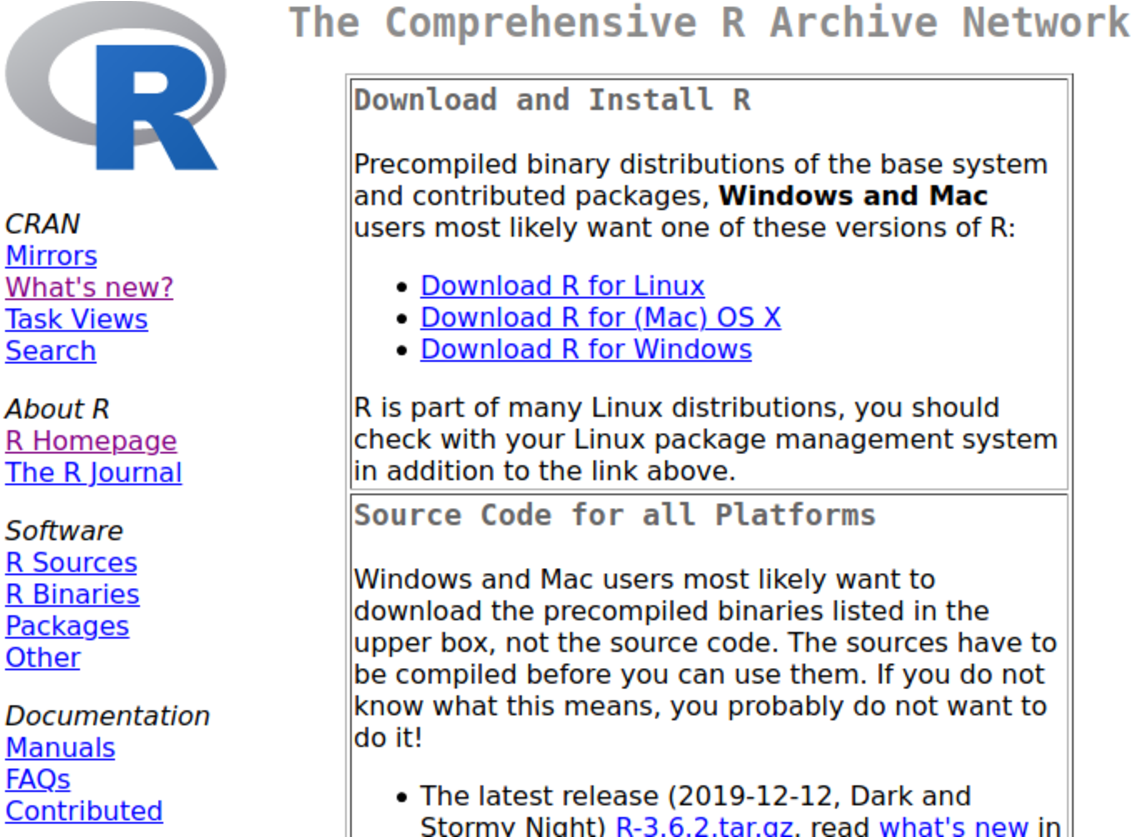
\includegraphics[width=0.6\linewidth]{cran}
    \label{fig:cran}
  \end{figure}

\end{frame}

\subsection{RjpWiki}

\myffr

  日本語での\R の情報源としては,次のウェブサイトが有名\\
  多くの有用な情報が掲載されており,質問もできる.\\
  $\rightarrow$ RjpWiki(\url{http://www.okadajp.org/RWiki})

  \begin{figure}[h]
    \centering
    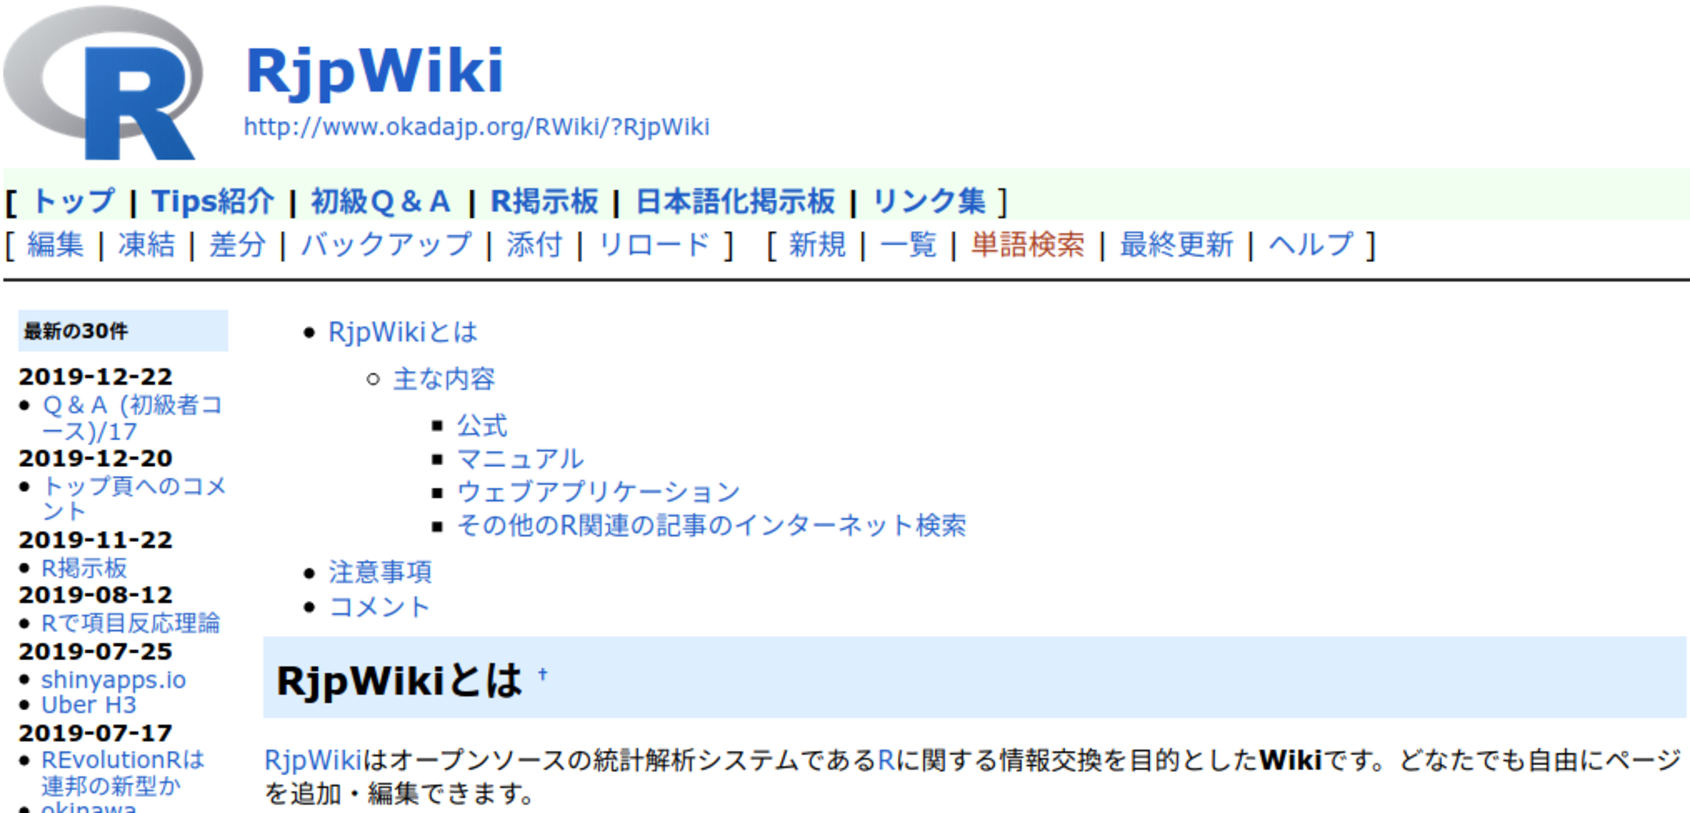
\includegraphics[width=0.9\linewidth]{rjpwiki}
    \label{fig:rjpwiki}
  \end{figure}

\end{frame}

\subsection{\RStudio}

\myffr

  \RStudio とは,\R 用の統合開発環境(IDE)で,
  ソースコードの編集,実行,ヘルプの表示,パッケージの作成など,
  プログラミングに必要な様々な便利な機能を持つソフトウェア
  \vspace{3mm}
  \begin{minipage}{0.45\hsize}
    \begin{figure}[h]
      \centering
      
\includegraphics[width=0.8\linewidth]{logo-rstudio}
      \label{fig:logo-rstudio}
    \end{figure}
  \end{minipage}
  \hspace{3mm}
  \begin{minipage}{0.45\hsize}
    \begin{figure}[h]
      \centering
      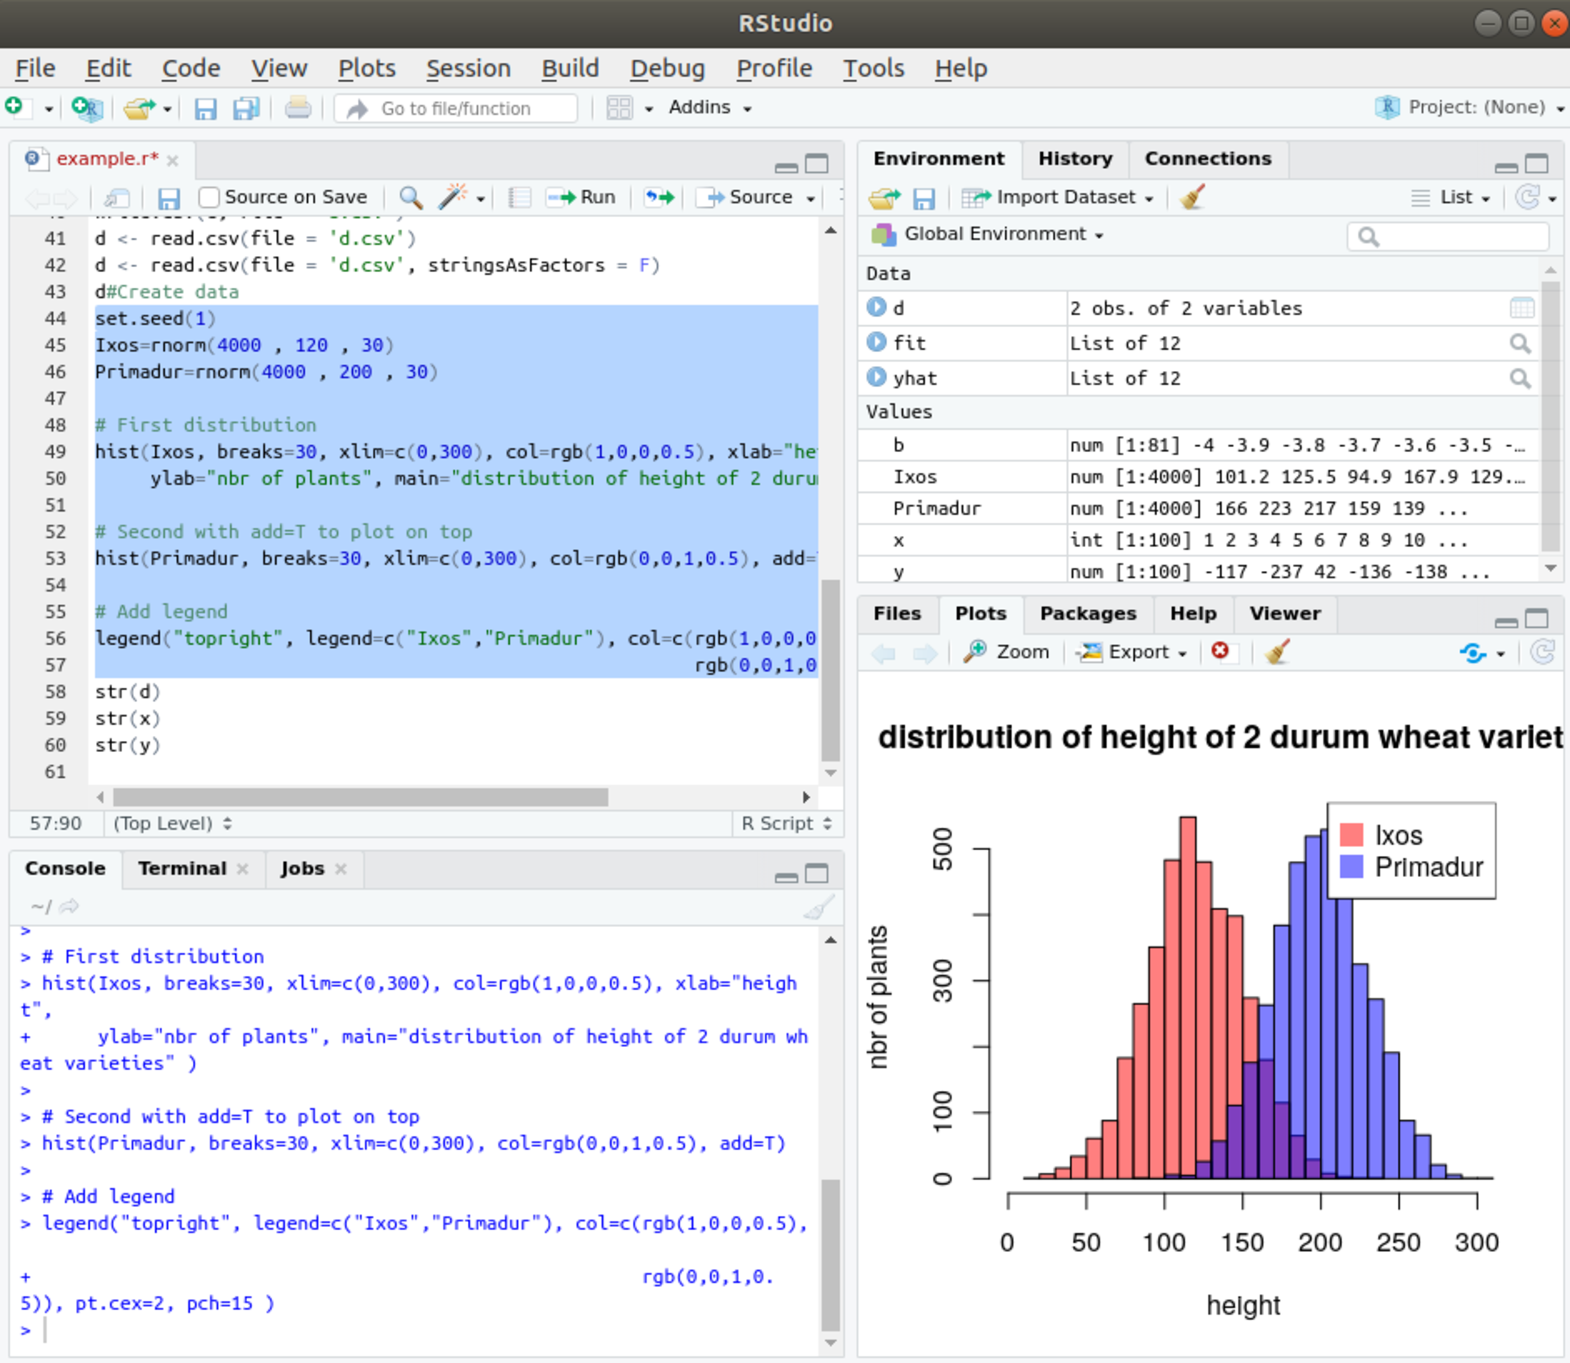
\includegraphics[width=0.9\linewidth]{rstudio}
      \label{fig:rstudio}
    \end{figure}
  \end{minipage}

  \vspace{5mm}
  オープンソース版の\RStudio を次のサイトからダウンロードできる. 
  $\rightarrow$ rstudio.com(\url{https://rstudio.com})

\end{frame}

\end{document}



\section{基本操作}
%
% Section title page as a seperator
%

\def\MyCourse{データサイエンスコース}
\def\MySubject{R入門}
\def\MySemester{春学期}

\newcommand{\R}{\textbf{R}}
\newcommand{\RStudio}{\textbf{RStudio}}
\newcommand{\Excel}{\textbf{Excel}}
\newcommand{\cs}[1]{\textcolor{blue}{\texttt{#1}}} % Console prompt >


\begin{frame}[fragile]
  \centering
  \Huge
  \insertsection 

\end{frame}

\end{document}


\def\MyCourse{データサイエンスコース}
\def\MySubject{R入門}
\def\MySemester{春学期}

\newcommand{\R}{\textbf{R}}
\newcommand{\RStudio}{\textbf{RStudio}}
\newcommand{\Excel}{\textbf{Excel}}
\newcommand{\cs}[1]{\textcolor{blue}{\texttt{#1}}} % Console prompt >


\subsection{スカラの作成}

\myffr

  \mybfr{手順}
    オブジェクト名の後に,代入(付置)記号「<-」と値を入力する.
  \mybto
・「<-」の代わりに「=」も使用できる (若干意味が異なる).\\
・オブジェクト名は,大文字と小文字は区別される.
  %・ls()で作成したオブジェクトの名前を表示できる.\\
  %・rm('x')でオブジェクトxを削除できる. rm(list=ls())で全消去.\\

  \myee
  {コンソール1}
  {
    \cs{x <- 1}\\
    \cs{kw.pv <- 3.1}
  }
  {コンソール2}
  {
    \cs{ls()} \mycheck{オブジェクト名表示}\\
    \cs{rm(list=ls())} \mycheck{全消去}
  }

%  \R ではオブジェクト名称の大文字と小文字は区別される.
%  漢字名称も使用可能だが,通常はローマ字小文字で,
%  判別可能な略語を用い,ofの意味で「.」や「\_」
%  を利用し単語を結合すると分かりやすくなる.
%  【例】lat.jp (日本の緯度),kw.pv(PV発電量)

  \mybfr{演習}
    「Alt~+~-」で代入記号(<-)を20回入力してください.\\
    オブジェクト名を表示,オブジェクトを削除してください.
  \mybto

\end{frame}

\end{document}


\def\MyCourse{データサイエンスコース}
\def\MySubject{R入門}
\def\MySemester{春学期}

\newcommand{\R}{\textbf{R}}
\newcommand{\RStudio}{\textbf{RStudio}}
\newcommand{\Excel}{\textbf{Excel}}
\newcommand{\cs}[1]{\textcolor{blue}{\texttt{#1}}} % Console prompt >


\subsection{ベクトルの作成}
\myffr

\mybbb
{手順(方法1)}{結合関数「c」を用いて作成}
{手順(方法2)}{等差数列作成記号「:」を用いて作成}
{手順(方法3)}{等差数列作成関数「seq」を用いて作成}\\[1mm]

「rep」関数で同一値ベクトル作成も可能
rep(NA, 3) $\rightarrow$ NA NA NA\\

「?関数名」をコンソールに入力するとヘルプが表示される.


\myeee
{コンソール1}{\cs{v <- c(1,6,3)}\\   \relax [1] 1 6 3}
{コンソール2}{\cs{v <- 1:3}\\        \relax [1] 1 2 3}
{コンソール3}{\cs{v <- seq(1,6,2)}\\ \relax [1] 1 3 5}\\[1mm]


\myb{演習}{
 次のベクトルを作成してください.\\
 「3 2 1」,「3 6 9」,「4 2 0」,「1.5 2.5 3.5」,「1 2 3 1 2 3」
}

\end{frame}

\end{document}


\def\MyCourse{データサイエンスコース}
\def\MySubject{R入門}
\def\MySemester{春学期}

\newcommand{\R}{\textbf{R}}
\newcommand{\RStudio}{\textbf{RStudio}}
\newcommand{\Excel}{\textbf{Excel}}
\newcommand{\cs}[1]{\textcolor{blue}{\texttt{#1}}} % Console prompt >


\subsection{行列の作成}
\myffr

  \mybfr{手順}
    行列作成関数「matrix」を用いて作成.行数:nrow,列数:ncol
  \mybto

  \myefr{コンソール}
    \cs{m <- matrix(1:4, nrow = 2, ncol = 2)}\\
    \hfill (オプション byrow = T で行毎に値代入)\\
    \cs{m}\\
    \vspace{-9mm}
    \begin{verbatim}
             [,1] [,2]
        [1,]    1    3
        [2,]    2    4
    \end{verbatim}
    \vspace{-9mm}
  \myeto

  \mybfr{演習}
    次の行列を作成してください.
    \vspace{-9mm}
    \[
      \hspace{40mm}
      \begin{bmatrix}
        -2 & 0 & 2\\
         4 & 6 & 8 
      \end{bmatrix}
      , 
      \begin{bmatrix}
        NA & NA\\
        NA & NA 
      \end{bmatrix}
    \]
  \mybto

\end{frame}

\end{document}


\def\MyCourse{データサイエンスコース}
\def\MySubject{R入門}
\def\MySemester{春学期}

\newcommand{\R}{\textbf{R}}
\newcommand{\RStudio}{\textbf{RStudio}}
\newcommand{\Excel}{\textbf{Excel}}
\newcommand{\cs}[1]{\textcolor{blue}{\texttt{#1}}} % Console prompt >


\subsection{オブジェクトの画面表示}

\myffr

  \mybfr{手順}
  コンソールに表示させたいオブジェクト名を入力する.
  または,ソースコード画面でオブジェクトを選択してCtrl+Enterを押す.
  \mybto 

  \myeee
    {コンソール1}
    {
      \cs{v[3]}\\ \relax
      [1] 3
    }
    {コンソール2}
    {
      \cs{m[2, ]}\\ \relax
      [1] 2 4
    }
    {コンソール3}
    {
      \cs{(x <- c(1, 2))}\\ \relax
      [1] 1 2
    }\\[1mm]

  【オブジェクト要素の\R 表記】\\
   ~~ベクトルvの要素$i$: v[i]\\
   ~~行列mの$i$行: m[i, ],$j$列: m[, j],要素$(i, j)$: m[i, j]

  \mybfr{演習}
    スカラ,ベクトル,行列の値を表示させてください.
  \mybto
  
\end{frame}

\end{document}


\def\MyCourse{データサイエンスコース}
\def\MySubject{R入門}
\def\MySemester{春学期}

\newcommand{\R}{\textbf{R}}
\newcommand{\RStudio}{\textbf{RStudio}}
\newcommand{\Excel}{\textbf{Excel}}
\newcommand{\cs}[1]{\textcolor{blue}{\texttt{#1}}} % Console prompt >


\subsection{データフレームの作成}

\myffr

  \mybfr{手順}
    テーブル作成関数「data.frame」を用いて作成する.
  \mybto

  \myefr{コンソール}
    \cs{d <- data.frame(name = c('panda', 'lion'),\\\hfill age  = c(5, 7), male = c(T, F))}\\
    \cs{d}\\
       ~~~name age  male\\
     1 panda   5  TRUE\\
     2 ~~~lion   7 FALSE\\
  \myeto

  \mybfr{演習}
    漢字,数値,論理値のカラムを持つ,
    データフレームを作成してください(内容自由).
  \mybto

\end{frame}

\subsection{データフレームの操作1}

\myffr

  \vspace{-4mm}

  \mybfr{手順}
    アクセスしたいコラム(列)やレコード(行)のインデック番号を入力する.
    負の番号を入れると,そのコラムが除かれる.
  \mybto

  \myeee
  {コンソール1}
  {
    \cs{ d[, 1] }\\ \relax
    [1] "panda" "lion" 
  }
  {コンソール2}
  {
    \cs{ d[, c(1, 3)] }\\
    ~~name  male\\
    1 panda  TRUE\\
    2 ~~~lion FALSE
  }
  {コンソール3}
  {
    \cs{ d[, -1] }\\
    ~~age  male\\
    1   5  TRUE\\
    2   7 FALSE
  }

  \mybfr{演習}
    レコード(行)にもインデックス番号でアクセスし,値の表示や代入を行ってください.
  \mybto

\end{frame}

\subsection{データフレームの操作2}

\myffr

  \vspace{-2mm}

  \mybfr{手順}
    オブジェクト名のあとにアクセスしたいコラム(列)名を$で結びつける.
    または,コラム(列)名をリテラルで囲み記入する.\\
    データフレームdのカラム: d\$カラム名 or d[, 'カラム名']
  \mybto

  \vspace{-2mm}

  \myee
    {コンソール1}
    {
      \cs{ d\$age }\\ \relax
      [1] 5 7
    }
    {コンソール2}
    {
      \cs{ d[, c('name', 'age')] }\\
      ~~~name age\\
        1 panda   5\\
        2 ~~~lion   7
    }

  \mybfr{演習}
  レコード(行)にもレコード名でアクセスし,値の表示や代入を行ってください.
  \mybto

  カラム名,レコード名はrownames(d), colnames(d)でアクセス可能
\end{frame}

\subsection{データフレームの操作3}

\myffr

  \mybfr{手順}
    アクセスしたいコラム(列)やレコード(行)に論理値を入力する.
    T(TRUE)の論理値箇所のデータが抽出される.
  \mybto

  \myee
    {コンソール1}
    {
      \cs{ d[, c(T, F, T)] }\\
          ~~~name  male\\
        1 panda  TRUE\\
        2 ~~~lion FALSE
    }
    {コンソール2}
    {
      \cs{ d[d\$age > 6, ] }\\
       ~~name age  male\\
       2 ~~lion ~~7 FALSE
     }

  \mybfr{演習}
    レコード(行)に論理値ベクトルでアクセスし,値の表示や代入を行ってください.
  \mybto

\end{frame}

\end{document}



\section{演算}
%
% Section title page as a seperator
%

\def\MyCourse{データサイエンスコース}
\def\MySubject{R入門}
\def\MySemester{春学期}

\newcommand{\R}{\textbf{R}}
\newcommand{\RStudio}{\textbf{RStudio}}
\newcommand{\Excel}{\textbf{Excel}}
\newcommand{\cs}[1]{\textcolor{blue}{\texttt{#1}}} % Console prompt >


\begin{frame}[fragile]
  \centering
  \Huge
  \insertsection 

\end{frame}

\end{document}


\def\MyCourse{データサイエンスコース}
\def\MySubject{R入門}
\def\MySemester{春学期}

\newcommand{\R}{\textbf{R}}
\newcommand{\RStudio}{\textbf{RStudio}}
\newcommand{\Excel}{\textbf{Excel}}
\newcommand{\cs}[1]{\textcolor{blue}{\texttt{#1}}} % Console prompt >


\subsection{四則}

\myffr

  \mybfr{手順}
    和「+」,減「-」,積「*」,除「/」,乗「\^\ 」,
    剰余「\%\%」,剰商「\%/\%」の算法記号を使って演算する.
    要素ごとの演算となる.
  \mybto
  この他,行列演算用の積「\%*\%」,転置「t()」,逆行列「solve()」などもある.

  \myeee
  {コンソール1}
  {
    \cs{x <- 1:3; y <- 1:3}\\
    \cs{x + y}\\ \relax
    [1] 2 4 6
  }
  {コンソール2}
  {
    \cs{x <- 1:3; y <- 1:3}\\
    \cs{x * y}\\ \relax
    [1] 1 4 9
  }
  {コンソール3}
  {
    \cs{x <- 9; y <- 2}\\
    \cs{x \%/\% y}\\ \relax
    [1] 4
  }

  \mybfr{演習}
    上記,すべての演算記号を使って,計算してください(内容自由).
  \mybto
  
\end{frame}

\subsection{組込関数1}

\myffr

  \mybfr{手順}
  平均値「mean」,中央値「median」,最大「max」,最小「min」\\
  範囲「range」,平方根「sqrt」,絶対値「abs」,丸め「round」など
  \mybto

  \myeee
  {コンソール1}
  {
    \cs{x <- 1:3}\\
    \cs{mean(x)}\\ \relax
    [1] 2
  }
  {コンソール2}
  {
    \cs{x <- 1:3}\\
    \cs{range(x)}\\ \relax
    [1] 1 3
  }
  {コンソール3}
  {
    \cs{x <- 3.14}\\
    \cs{round(x, 1)}\\ \relax
    [1] 3.1 
  }

  \mybfr{演習}
    上記,すべての組み込み関数を使って,計算してください(内容自由).
    また,その他の関数,定数(pi)は,どのようなものがあるかインターネットで検索してください.
  \mybto
  
\end{frame}

\subsection{組込関数2}

\myffr

  \mybfr{手順}
  平均値「mean」,中央値「median」,最大「max」,最小「min」\\
  範囲「range」,平方根「sqrt」,絶対値「abs」,丸め「round」など
  \mybto

  \myeee
  {コンソール1}
  {
    \cs{x <- 1:3}\\
    \cs{mean(x)}\\ \relax
    [1] 2
  }
  {コンソール2}
  {
    \cs{x <- 1:3}\\
    \cs{range(x)}\\ \relax
    [1] 1 3
  }
  {コンソール3}
  {
    \cs{x <- 3.14}\\
    \cs{round(x, 1)}\\ \relax
    [1] 3.1 
  }

  \mybfr{演習}
    上記,すべての組み込み関数を使って,計算してください(内容自由).
    また,その他の関数,定数(pi)は,どのようなものがあるかインターネットで検索してください.
  \mybto
  
\end{frame}

\subsection{自作関数1}
\myffr

  \mybfr{手順}
    関数オブジェクト名 <- function (引数1,引数2,...) 関数式\\
    の形式で関数を作成する.引数は値渡しとなる.
  \mybto

  \myefr{コンソール}
    \cs{get.mbe <- function(yhat, y) mean(yhat - y)}\\
    \cs{mbe <- get.mbe(yhat \textcolor{red}{=} 1:3, y \textcolor{red}{=} 4:6)}\\\relax
    [1] -3
  \myeto

  \mybfr{演習}
    RMSE(平均2乗誤差平方)を求める関数を作成してください.
    \vspace{-2mm}
    \[
    \mathrm{RMSE} = \sqrt{\frac{1}{N} \sum_{i = 1}^{N} (\hat{y}_i-y_i)^2}
    \hspace{5mm} \mbox{平均:mean(),平方根:sqrt()}
    \]
  \mybto
  
\end{frame}

\subsection{自作関数2}

\myffr

  \mybfr{手順}
    複数行の関数を作成するときは,関数のスコープを示す{}(中括弧)や変数名を指定して出力するreturn関数を用いる.
  \mybto 

  \myee
  {コンソール1}
  {
    \cs{f <- function(x) \{ \mycheck{}\\
        ~~~~~y~<- 1 + x + x \^ \ 2\\
        ~~~~~z~<- log(y)\\
        ~~~~~return(z) \mycheck{}\\
        ~~~\} \mycheck{}
    }
  }
  {コンソール2}
  {
    \cs{f(2)}\\\relax
    [1] 1.94591
  }\\[2mm]

  \mycheck{ return関数では,最後のオブジェクトを返す場合は記述しなくてもよい.}

  \mybfr{演習}
    複数行の関数を作成してください.
  \mybto
  
\end{frame}

\end{document}



\section{描画}
%
% Section title page as a seperator
%

\def\MyCourse{データサイエンスコース}
\def\MySubject{R入門}
\def\MySemester{春学期}

\newcommand{\R}{\textbf{R}}
\newcommand{\RStudio}{\textbf{RStudio}}
\newcommand{\Excel}{\textbf{Excel}}
\newcommand{\cs}[1]{\textcolor{blue}{\texttt{#1}}} % Console prompt >


\begin{frame}[fragile]
  \centering
  \Huge
  \insertsection 

\end{frame}

\end{document}


\def\MyCourse{データサイエンスコース}
\def\MySubject{R入門}
\def\MySemester{春学期}

\newcommand{\R}{\textbf{R}}
\newcommand{\RStudio}{\textbf{RStudio}}
\newcommand{\Excel}{\textbf{Excel}}
\newcommand{\cs}[1]{\textcolor{blue}{\texttt{#1}}} % Console prompt >


\subsection{描画用データ作成}

\myffr

\mybfr{手順}
描画用データとして,平均,標準偏差が異なる3種類の正規乱数(N=100)を作成する.
また,表示用の色をそれぞれ作成する.
\mybto

\begin{minipage}{0.45\hsize}

\lstinputlisting[firstline=1,lastline=21]{graph.r}

\end{minipage}
\hspace{3mm}
\begin{minipage}{0.5\hsize}
\mybfr{演習}
左のソースコードを「graph.r」として保存してください.\\
色彩名表示colors()でどのような色があるか確認してください.
%「R」,「色見本」,「colors」などのキーワードで,インターネットでどのような色見本があるか検索してください.
\mybto
\mycheck{\tiny 色彩名 -> RGB変換: col2rgb('色彩名')}\\
\mycheck{\tiny 色彩名関数: rainbow(n), heat.colors(n), grey(1:11/12),\\\hfill terrain.colors(n), topo.colors(n), cm.colors(n)}\\
\mycheck{\tiny cf. \href{https://oku.edu.mie-u.ac.jp/~okumura/stat/colors.html}{奥村研究室,「統計グラフの色」}}
\end{minipage}

\end{frame}

\subsection{散布図}

\myffr

\begin{minipage}{0.45\hsize}
\tiny
\vspace{-3mm}
\lstinputlisting[language=R, firstline=3,lastline=21]{050-scatter.r}

\mybfr{演習}
グラフィックオプションは次のようなものがあります.\\
値を変更してグラフを変化させてみてください.\\ \relax
type=\{p, l, b, o, s, h, n\}, pch=0--25, lty=0--6
\mybto

\end{minipage}
\hspace{3mm}
\begin{minipage}{0.45\hsize}
\begin{figure}[t]
  \centering
  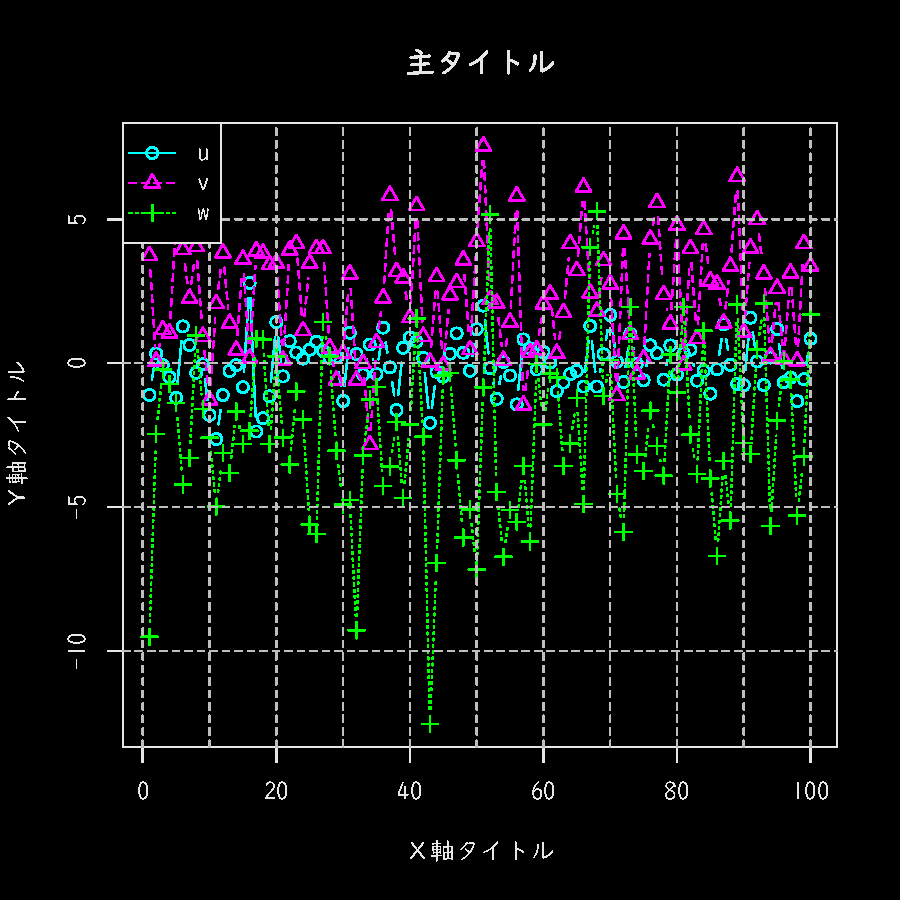
\includegraphics[width=\hsize]{fig/scatter}
  \caption{散布図描画例}
  \label{fig:scatter}
\end{figure}
\vspace{-5mm}

\mycheck{\tiny{type: plot \textbf{type}, col: plot \textbf{col}or, bg: \textbf{b}ack\textbf{g}round color}}\\
\mycheck{\tiny{pch: \textbf{p}oint \textbf{ch}aracter, lty: \textbf{l}ine \textbf{ty}pe, lwd: \textbf{l}ine \textbf{w}i\textbf{d}th}}\\
\mycheck{\tiny{h: \textbf{h}orizontal line, v: \textbf{v}ertical line}}\\

\end{minipage}

\end{frame}

\subsection{ヒストグラム}

\myffr

\begin{minipage}{0.45\hsize}
\tiny
\vspace{-3mm}
\lstinputlisting[language=R, firstline=3,lastline=26]{050-hist.r}

\end{minipage}
\begin{minipage}{0.45\hsize}
\begin{figure}[t]
  \centering
  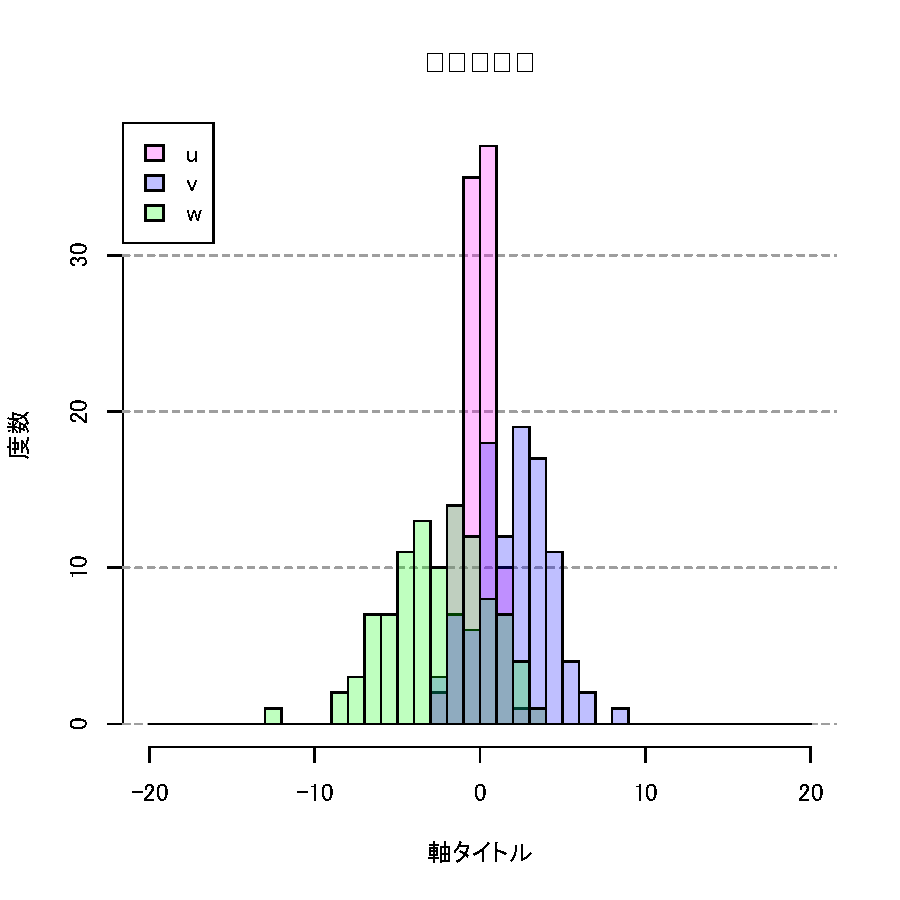
\includegraphics[width=\hsize]{fig/hist}
  \caption{ヒストグラム描画例}
  \label{fig:hist}
\end{figure}
\vspace{-5mm}
\mycheck{\tiny{add = T オプションで重ね書きができる}}\\
\mycheck{\tiny{rgb(red = 0, blue = 1, green = 0, alpha = .5)\\
               \hfill でRGB値を出力できる(alpha: 透明度)}}\\

\end{minipage}

\end{frame}

\subsection{回帰モデルグラフ}

\myffr

\begin{minipage}{0.50\hsize}
\tiny
\vspace{-3mm}
\lstinputlisting[language=R, firstline=3,lastline=28]{051-lm-plot.r}
\vspace{-4mm}
\normalsize
\end{minipage}
\begin{minipage}{0.45\hsize}

\begin{figure}[t]
  \centering
  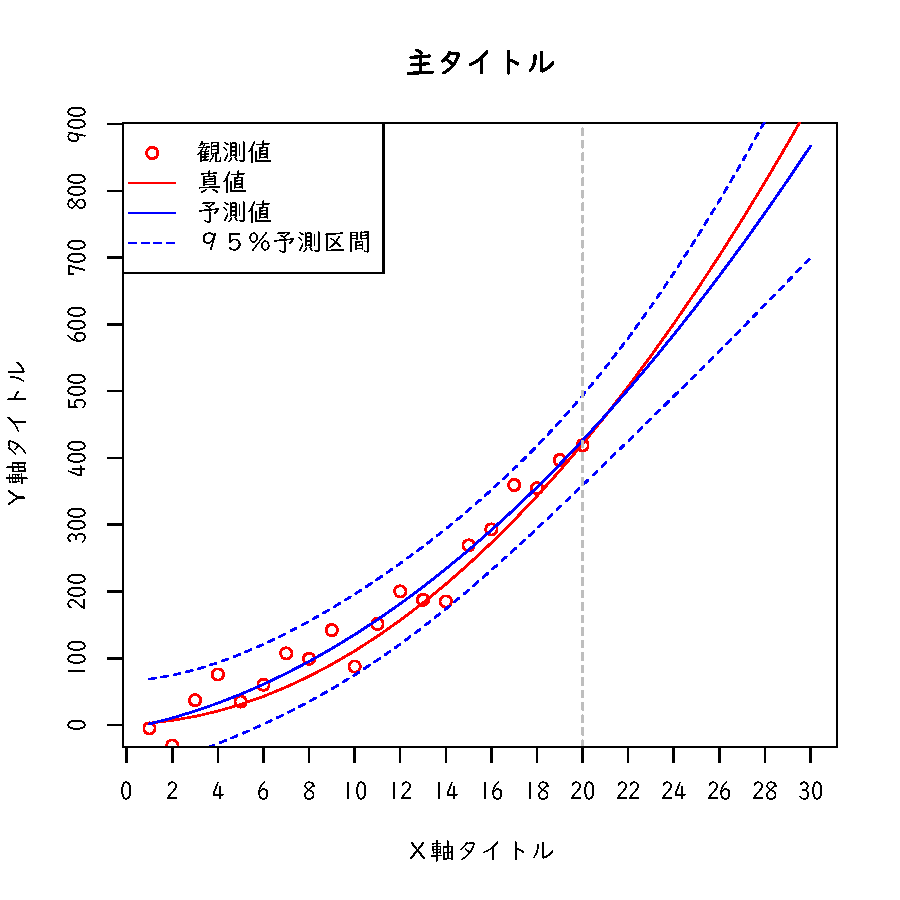
\includegraphics[width=\hsize]{fig/lm}
  \caption{回帰モデルグラフ描画例}
  \label{fig:lm}
\end{figure}
\vspace{-8mm}
\mycheck{描画関数\tiny{matpoints: 点,matlines: 線,abline: 縦横線,axis: 軸,legend: 凡例}}\\
\mycheck{描画オプション\tiny{col: 色,pch: 点種,lty: 線種,v:縦線,h:横線}}

\end{minipage}

\end{frame}

\end{document}



\section{入出力}
%
% Section title page as a seperator
%

\def\MyCourse{データサイエンスコース}
\def\MySubject{R入門}
\def\MySemester{春学期}

\newcommand{\R}{\textbf{R}}
\newcommand{\RStudio}{\textbf{RStudio}}
\newcommand{\Excel}{\textbf{Excel}}
\newcommand{\cs}[1]{\textcolor{blue}{\texttt{#1}}} % Console prompt >


\begin{frame}[fragile]
  \centering
  \Huge
  \insertsection 

\end{frame}

\end{document}


\def\MyCourse{データサイエンスコース}
\def\MySubject{R入門}
\def\MySemester{春学期}

\newcommand{\R}{\textbf{R}}
\newcommand{\RStudio}{\textbf{RStudio}}
\newcommand{\Excel}{\textbf{Excel}}
\newcommand{\cs}[1]{\textcolor{blue}{\texttt{#1}}} % Console prompt >


\subsection{テキストデータの出力}

\myffr

  \mybfr{手順}
    write.csv関数を使用して,オブジェクトデータを
    ファイルにCSVファイル形式*で書き込む.
    * CSV:カンマ区切
  \mybto
  

  \myefr{コンソール}
    \cs{ d0 <- data.frame(name = c('panda', 'lion'), age = c(5, 7)) }\\
    \cs{ write.csv(d0, file = 'd0.csv') }
  \myeto

  quote = Fオプションをつけると文字列引用符「"」を削除できる.
  write.csv(d0, file = 'd0.csv', quote = F)

  \mybfr{演習}
    データフレームを作成し,ファイルに出力してください.
  \mybto

\end{frame}

\subsection{テキストデータの入力}

\myffr

  \mybfr{手順}
    read.csv関数を使用して,CSVファイルを読み込み
    オブジェクトに格納する.
  \mybto

  \myefr{コンソール}
    \cs{d1 <- read.csv(file = 'd0.csv')}\\
    \cs{str(d1)}
  \myeto

  stringsAsFactors = Fオプションをつけると文字列の自動因子化を抑制します.
  read.csv(file = 'd0.csv', stringsAsFactors = F)

  \mybfr{演習}
    CSVファイルを読み込み,オブジェクトに格納してください.
  \mybto

\end{frame}

\subsection{\Excel データの入力}

\myffr

  \mybfr{手順}
    excel.linkパッケージを利用し,\R とリンクさせる.\\
    パッケージの利用コマンド: library(excel.link)
  \mybto

  \myefr{コンソール}
    \cs{library(excel.link)}\\
    \cs{xl.workbook.open('test.xlsx')}\hfill \mycheck{Excelを開く}\\
    \cs{d <- data.frame(x=3:1, y=-1:1)}\\
    \cs{xl['Sheet1!A1'] <- d}\hfill \mycheck{Sheet1のA1を起点としてデータを書き込み}\\
    \cs{xl['Sheet1!B2'] -> x}\hfill \mycheck{Sheet1のB2からデータを読み込み}\\
    \cs{xl.workbook.save('test.xlsx')}\hfill \mycheck{Excelを保存}
  \myeto

  \mycheck{xlr: 行名付き,xlc:列名付き, xlrc:行列名付き入出力}

  \mybfr{演習}
    パッケージのヘルプにあるサンプルコードを用いてExcelを操作してください.
  \mybto

\end{frame}

\end{document}



\section{統計解析}
%
% Section title page as a seperator
%

\def\MyCourse{データサイエンスコース}
\def\MySubject{R入門}
\def\MySemester{春学期}

\newcommand{\R}{\textbf{R}}
\newcommand{\RStudio}{\textbf{RStudio}}
\newcommand{\Excel}{\textbf{Excel}}
\newcommand{\cs}[1]{\textcolor{blue}{\texttt{#1}}} % Console prompt >


\begin{frame}[fragile]
  \centering
  \Huge
  \insertsection 

\end{frame}

\end{document}


\def\MyCourse{データサイエンスコース}
\def\MySubject{R入門}
\def\MySemester{春学期}

\newcommand{\R}{\textbf{R}}
\newcommand{\RStudio}{\textbf{RStudio}}
\newcommand{\Excel}{\textbf{Excel}}
\newcommand{\cs}[1]{\textcolor{blue}{\texttt{#1}}} % Console prompt >


\subsection{観測データと試験データの作成}

\myffr

  \mybfr{手順}
    観測値,時刻データ(1--20),予測対象時刻データ(21--30),
    全期間時刻データ(1--30)を作成する.\\
    現実的には,真値は分からないがこれも作成する.
  \mybto

  \myefr{コンソール}
    \myon{1,7}
    \cs{n.obs <- 20; n.fct <- 10; n.all <- n.obs + n.fct} \hfill \mycheck{データサイズ}\\
    \myon{2,7}
    \cs{x.obs <- 1:n.obs; x.all <- 1:n.all}      \hfill \mycheck{観測時刻;全時刻}\\
    \myon{3,7}
    \cs{f <- function(x) 1 + x + x \^ \ 2}       \hfill \mycheck{真のモデル}\\
    \myon{4,7}
    \cs{e <- rnorm(n = n.obs, sd = 30)}          \hfill \mycheck{観測ノイズ}\\
    \myon{5,7}
    \cs{y.obs~ <- f(x.obs) + e}                  \hfill \mycheck{観測値}\\
    \myon{6,7}
    \cs{y.true <- f(x.all)}                      \hfill \mycheck{真値}
    \myon{7}

  \myeto

  \mybfr{演習}
    どのような値が入っているか確認してください.
  \mybto
  
\end{frame}

\subsection{学習(フィッティング)}

\myffr

  \mybfr{手順}
    lm関数を用いて線形モデルのフィッティングを行う.
    変数の加工は\texttt{I()}で囲む.切片は標準でモデルに入っている.
  \mybto

  \myefr{コンソール}
  \cs{fit <- lm('y \~\ x + I(x\^\relax 2)', data=data.frame(x=x.obs, y=y.obs))}\\
  \cs{summary(fit)}\\
    \vspace{-5mm}
\begin{verbatim}
             Estimate Std. Error t value Pr(>|t|)
 (Intercept)   1.8203    25.8913   0.070    0.945
 x            -4.7082     5.6784  -0.829    0.419
 I(x^2)        1.3641     0.2627   5.194 7.32e-05 ***
\end{verbatim}
    \vspace{-3mm}
  \myeto

  \mycheck{\texttt{Estimate}: 回帰係数推定値},\mycheck{\texttt{Pr(>|t|)}: p値(星屑が付いていれば有意)}

  \mybfr{演習}
    モデル y \~ \ x + I(x \^ \ 2) を変えて,フィッティングしてください.
  \mybto
  
\end{frame}

\subsection{予測}

\myffr

  \mybfr{手順}
    predict関数(正式名:predict.lm)を用いて未来予測を行う.
  \mybto

  \myefr{コンソール}
    \cs{m <- predict(fit, newdata = data.frame(x = x.all),\\
    \hfill interval = 'prediction', level = 0.95)} \\
    \cs{tail(m, 2)}
    \vspace{-5mm}
      \begin{verbatim}
              fit      lwr      upr
      29 1012.4739 818.1671 1206.781
      30 1088.2464 874.4287 1302.064
      \end{verbatim}
    \vspace{-8mm}
  \myeto

  \mycheck{interval: 区間推定種類,level: 信頼水準}\\
  \mycheck{fit:予測値,lwr:下限値,upr:上限値} \mycheck{tail: 末尾データ閲覧関数(cf. head)}

  \mybfr{演習}
   区間の種類(信頼区間:confidence,予測区間:prediction)や信頼水準(level)を変えて値がどう変化するか確認してください.
  \mybto
  
\end{frame}

\subsection{回帰モデルグラフ}

\myffr

\begin{minipage}{0.50\hsize}
\tiny
\vspace{-3mm}
\lstinputlisting[language=R, firstline=3,lastline=28]{061-lm-plot.r}
\vspace{-4mm}
\normalsize
\end{minipage}
\begin{minipage}{0.45\hsize}

\begin{figure}[t]
  \centering
  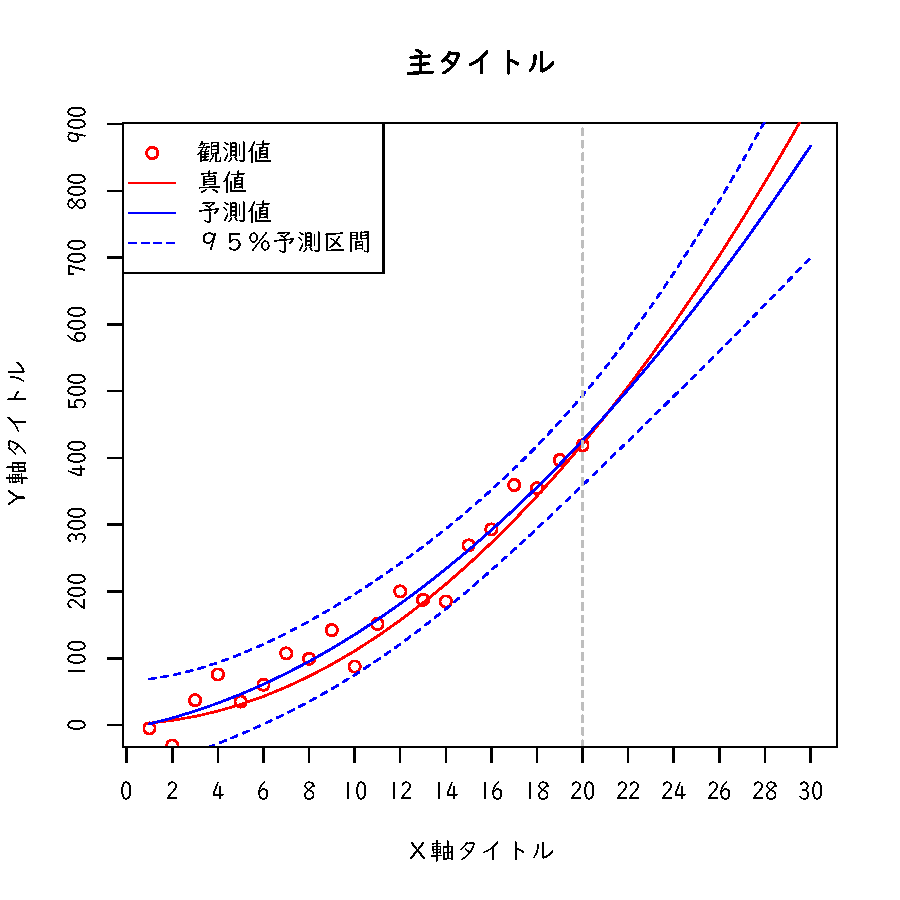
\includegraphics[width=\hsize]{fig/lm}
  \caption{回帰モデルグラフ描画例}
  \label{fig:lm60}
\end{figure}
\vspace{-8mm}
\mycheck{描画関数\tiny{matpoints: 点,matlines: 線,abline: 縦横線,axis: 軸,legend: 凡例}}\\
\mycheck{描画オプション\tiny{col: 色,pch: 点種,lty: 線種,v:縦線,h:横線}}

\end{minipage}

\end{frame}

\end{document}



\section{おわりに}
\def\MyCourse{データサイエンスコース}
\def\MySubject{R入門}
\def\MySemester{春学期}

\newcommand{\R}{\textbf{R}}
\newcommand{\RStudio}{\textbf{RStudio}}
\newcommand{\Excel}{\textbf{Excel}}
\newcommand{\cs}[1]{\textcolor{blue}{\texttt{#1}}} % Console prompt >


\mysffr

\R は統計解析だけでなく,業務効率化のソフトウェアツールとして幅広く活用できます.\\[3mm]

本ワークショップに参加された皆様のアイディアにより業務効率化が今後一層進むことを楽しみにしています.

\end{frame}

\end{document}



\appendix

%
% Appendix
%

\def\MyCourse{データサイエンスコース}
\def\MySubject{R入門}
\def\MySemester{春学期}

\newcommand{\R}{\textbf{R}}
\newcommand{\RStudio}{\textbf{RStudio}}
\newcommand{\Excel}{\textbf{Excel}}
\newcommand{\cs}[1]{\textcolor{blue}{\texttt{#1}}} % Console prompt >


\begin{frame}[fragile]
  \centering
  \Huge
  付録 

\end{frame}

\end{document}



\section{インストール方法}
\def\MyCourse{データサイエンスコース}
\def\MySubject{R入門}
\def\MySemester{春学期}

\newcommand{\R}{\textbf{R}}
\newcommand{\RStudio}{\textbf{RStudio}}
\newcommand{\Excel}{\textbf{Excel}}
\newcommand{\cs}[1]{\textcolor{blue}{\texttt{#1}}} % Console prompt >


\mysffr
  \begin{enumerate}
    \item \R
    \item \RStudio
    \item \R パッケージ
  \end{enumerate} 
\end{frame}

\subsection{\R}
\myffr

  統計数理研究所(\url{https://cran.ism.ac.jp})のCRANミラーサイト
  から\R をダウンロードし,インストールする.

  \mybfr{手順}
  CRANのポータル画面より,次の順にリンクを進み,\\
  Windows版のインストーラをダウンロードし,実行する.\\
  「\textcolor{blue}{Download R for Windows}」$\rightarrow$
  「\textcolor{blue}{install R for the first time}」\\
  \mybto
  \vspace{5mm} 

  \begin{figure}[h]
    \centering
    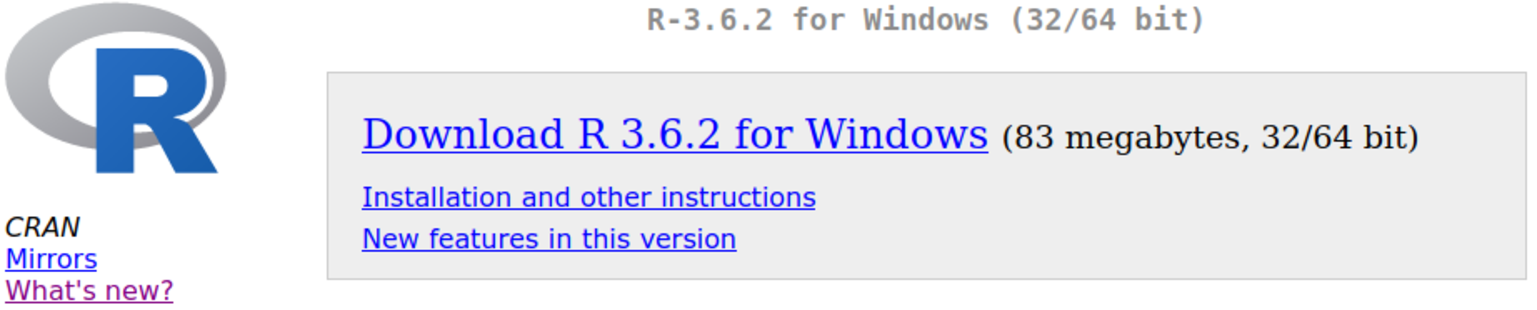
\includegraphics[width=\linewidth]{download-r}
    \label{fig:download-r}
  \end{figure}

\end{frame}

\subsection{\RStudio}

\myffr

  rstudio.com(\url{https://rstudio.com})から
  オープンソース版の\RStudio をダウンロードし,インストールする.

  \mybfr{手順}
    次のURLで「RStudio Desktop」の「DOWNLOAD」ボタンを押し,
    Windows版のインストーラをダウンロードし,実行する.
    \url{https://rstudio.com/products/rstudio/download}
  \mybto

  \vspace{1mm} 

  \begin{figure}[h]
    \centering
    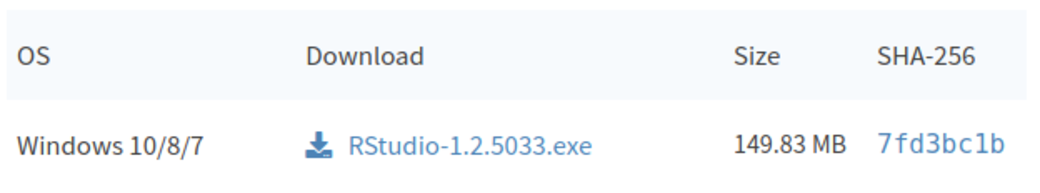
\includegraphics[width=\linewidth]{installer-rstudio}
    \label{fig:installer-rstudio}
  \end{figure}

\end{frame}

\myffr

\framesubtitle{CRANミラーサイト設定}

  デフォルトのCRANミラーサイトを国内サイト\\
  「41: Japan (Tokyo) [https]」に変更する.

  \mybfr{手順}
    コンソールで「chooseCRANmirror()」を入力し,\\
    「Selection:」のプロンプトが表示されたら「41」を入力する.
  \mybto

  \myefr{コンソール}
    \cs{chooseCRANmirror()}
    Secure CRAN mirrors\\
    \hspace{1mm}1: 0-Cloud [https]\\
    \hspace{1mm}2: Algeria [https]\\               
    \hspace{1mm}:\\               
    \textcolor{blue}{Selection: 41}
  \myeto

\end{frame}

\subsection{\R パッケージ}

\myffr

  \mybfr{手順}
    コンソールで「install.packages('***')」を入力する.\\
    ***には,インストールしたい\R パッケージ名が入る.
  \mybto

  \myefr{コンソール}
    \cs{install.packages('excel.link')}
  \myeto

  【注意】\\
  社内標準PCからは,この方法では\R パッケージを
  ダウンロードできない.
  対処方法としては,
  標準外PCで予めダウンロードし,
  \R インストールディレクトリ¥library内にある
  \R パッケージ,および,
  そのパッケージが依存するすべてのパッケージ
  (同一タイムスタンプで判別)を
  USBで標準PCのlibrary内にコピーする.

\end{frame}

\end{document}



\setbeamertemplate{headline}{}

\begin{frame}[fragile]
  \centering
  \Huge{END}
  %\hfill Last revised on: 2020-02-21.

\end{frame}

\end{document}

